\chapter{Objetivos del proyecto}

%\newpage
%Objetivos, alcance, planificación temporal, herramientas, 
%gestión de riesgos, evaluación económica

\section{Objetivos}
Los objetivos del proyecto consisten en crear un software que extienda la funcionalidad actual del sistema INTRASIM desarrollado 
por la universidad de Navarra y del grupo de investigación GALAN perteneciente a la UPV/EHU.

El software, debe permitir cargar observaciones y propiedades previamente capturadas con diversos
sistemas interactivos (por ejemplo, con un dispositivo Kinect) y
visualizarlas gr\'aficamente. Esas observaciones y propiedades se cargar\'an en un panel lateral con forma de \'arbol
y podr\'an seleccionarse para ser visualizadas. Los gr\'aficos pueden ser reorganizados como el
usuario quiera, para verlos al mismo tiempo.

La herramienta ha de permitir la visualizaci\'on de esas observaciones y propiedades. 
Tambi\'en permitir\'a la reproducci\'on de v\'ideos (si est\'an disponible).
El fin de la herramienta es
facilitar al usuario experto la identificaci\'on de intervalos donde se producen los
pasos y situaciones para posteriormente extraer de manera semiautom\'atica las relaciones entre las observaciones y
propiedades que forman parte de cada paso o situaci\'on.

\section{Alcance}
Se ha decidido utilizar las metodolog\'ias
\'agiles de desarrollo, como Scrum y Kanban en detrimento de los desarrollos cl\'asicos 
como puede ser el desarrollo en cascada  
\footnote{\url{www.cs.umd.edu/class/spring2003/cmsc838p/Process/waterfall.pdf}}.
Al utilizar este tipo de metodolog\'ias se hace frente a uno de los mayores problemas del 
desarrollo de software: la incertidumbre y los cambios
no contemplados inicialmente, facilitando la reacci\'on ante los cambios
al ser mucho mas flexible.

Al utilizar un modelo de desarrollo \'agil, el ciclo de vida que va a utilizarse, ser\'a iterativo e incremental.

Antes de exponer el alcance, es necesario saber en que consiste Scrum y Kanban.

\subsection{Scrum}
Scrum es una serie de herramientas (framework) para la gesti\'on y desarrollo de software basado en un proceso iterativo e incremental 
\cite{Scrum:WhatIsIt}.

\begin{figure}[H]
	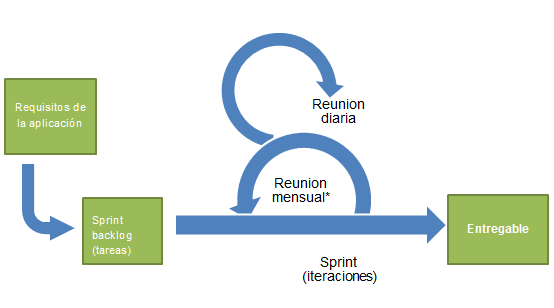
\includegraphics[width=0.7\linewidth]{./Figures/Scrumm.PNG}
	\caption[Proceso iterativo Scrum]{Diagrama Scrum}
	\label{fig:Scrum}
\end{figure}

En la figura \ref{fig:Scrum} \footnote{\url{https://upload.wikimedia.org/wikipedia/commons/e/e5/Scrumm.PNG} Autor: Maxie Ayala 
	Licenciado bajo \hyperlink{creativecommons.org/licenses/by-sa/3.0/}{CC BY-SA 3.0}} 
se puede ver el método de trabajo seg\'un Scrum, en el cual se observa lo importante que son los entregables.

%\newpage
Scrum, de manera resumida consiste en lo siguiente:
\begin{enumerate}
	\item Hablar con el cliente para ver si hay nuevos requisitos.
	\item Crear backlog, es decir, las tareas de ese sprint.
	\item Programar los requisitos especificados en el sprint.
	\item Reunión de retrospectiva para ver que ha ido mal y mejorarlo.
	\item Enviar entregable al cliente.
	\item Repetir.
\end{enumerate}

Es fundamental entre sprint y sprint que el valor del producto haya aumentado. Lo importante es el producto, no el 
avance del propio proyecto. Se podr\'ia avanzar mucho en el dise\~no del software, pero si eso es algo que el cliente no 
puede ver, se estar\'a fallando en el objetivo de ser \'agiles, ya que no le aporta nada.

Por otro lado, si se comete alg\'un error ser\'a muy sencillo corregirlo ya que si los sprints son de dos semanas por ejemplo, no 
se habr\'a perdido apenas tiempo. Y adem\'as para el cliente los entregables ser\'an predecibles en el tiempo, 
y se podr\'a estimar mejor cuando una funcionalidad presente en el \emph{backlog}
ser\'a introducida en el software. Esto \'ultimo es cierto porque se sabe la cantidad media de requisitos que se
entregan en cada sprint, por lo que se puede realizar una predicci\'on r\'apida y razonablemente precisa.

Scrum es tambi\'en muy interesante, y se posiciona como una alternativa muy potente frente a 
COCOMO o waterfall, porque en la creaci\'on de software hay un componente de incertidumbre muy 
grande. No se sabe c\'omo, ni cu\'ando pueden cambiar los requisitos de un 
software. Por ello, toman de nuevo importancia los sprints. 

En los modelos antiguos, si ya se hab\'ia terminado la fase de an\'alisis y dise\~no, y se requer\'ia una nueva funcionalidad era necesario 
paralizar el desarrollo del software y volver a analizar y diseñar. En cambio, con Scrum es 
posible integrar ese cambio en el siguiente sprint.

\subsection{Kanban}
Kanban es un m\'etodo de organizaci\'on del conocimiento del trabajo que se est\'a realizando con un gran \'enfasis en el la entrega justo a 
tiempo \footnote{JIT Delivery: Just-In-Time Delivery} sin sobrecargar al equipo \cite{Kanban:WhatIsIt}.

Kanban se centra mucho en que lo importante no es empezar muchas cosas, si no que se finalice
aquello que est\'a empezado. Sirve sobre todo 
para ver de una manera visual:
\begin{itemize}
	\item Qu\'e hay pendiente
	\item Qu\'e se est\'a haciendo ahora mismo
	\item Qu\'e se ha terminado.
\end{itemize}

El m\'{e}todo Kanban es algo muy extenso, pero en este proyecto, simplemente se ha aplicado el tablero Kanban mezclado con Scrum. 
Cada mes, se crea una lista de tareas que se debe completar (Sprint Backlog) y se coloca en la columna de ``Tareas pendientes", 
ordenadas por prioridad. Despu\'es, se coloca en la lista de ``En progreso" \ como m\'{a}ximo dos tareas. Y no se empieza ninguna otra
hasta que esas dos hayan sido pasadas a la columna de ``Tareas finalizadas".

\section{Descripci\'on de las tareas}
El alcance del proyecto va a definirse mediante un EDT, en el que se muestran las tareas de las
que se compone este TFG.

\begin{figure}[h]
	\centering
	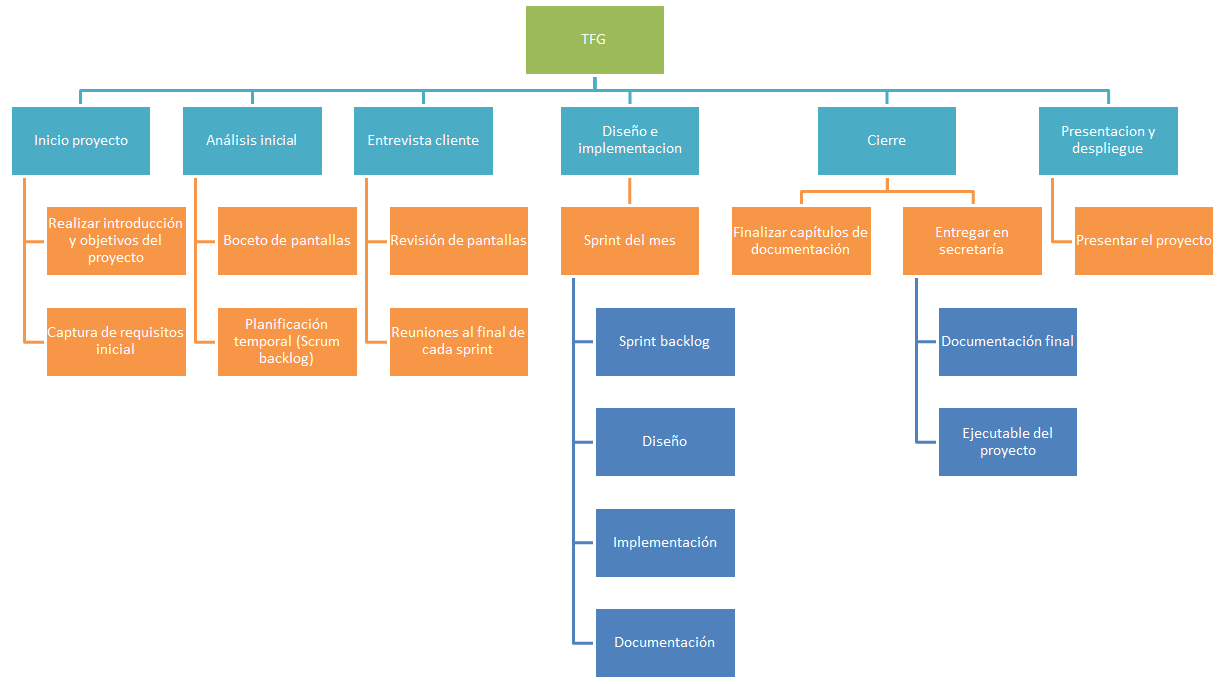
\includegraphics[width=1\linewidth]{./Figures/EDT}
	\caption[Alcance del proyecto]{EDT}
	\label{fig:Alcance}
\end{figure}
Tal y como se ve en la Figura \ref{fig:Alcance} cada una de las tareas de los grupos
``An\'alisis inicial", ``Entrevista cliente" \ y ``Dise\~no e implementaci\'on" \ van a realizarse en cada uno de los sprints.
Para cada tarea se ha realizado una peque\~na tabla en la que se detalla que se va a hacer,
la duraci\'on y esfuerzo aproximados, as\'i como otros datos de inter\'es.

\subsection{Inicio proyecto}
\subsubsection{Realizar introducci\'{o}n y objetivos del proyecto}
\begin{table}[H]
    \begin{center}
        \rowcolors{1}{lightgray}{} %\rowcolors{<starting row index>}{<odd row color>}{<even row color>}
        \begin{tabular}{l p{8cm}}
            Duraci\'{o}n (Horas / Persona)        & 7. \\ 
            Descripci\'{o}n                       & Realizar las secciones de la memoria de la Introducci\'{o}n y los
            objetivos del proyecto. \\
            Entradas                              & Scrum backlog  \\
            Salidas / Entregables                 & Los cap\'{i}tulos de introducci\'{o}n y objetivos del proyecto. \\
            Recursos necesarios                   & PC, \LaTeX, TeXStudio. \\
            Precedencias                          & Ninguna. \\
        \end{tabular}
    \end{center}
    
\end{table}

\subsubsection{Captura de requisitos inicial}
\begin{table}[H]
    \begin{center}
        \rowcolors{1}{lightgray}{} %\rowcolors{<starting row index>}{<odd row color>}{<even row color>}
        \begin{tabular}{l p{8cm}}
            Duraci\'{o}n (Horas / Persona)        & 7. \\ 
            Descripci\'{o}n                       & Entrevistarse con el cliente para obtener
                                                    una captura de requisitos inicial. \\
            Entradas                              & Ninguna. \\
            Salidas / Entregables                 & Diagrama de casos de uso y modelo de dominio. \\
            Recursos necesarios                   & PC, \LaTeX, TeXStudio. \\
            Precedencias                          & Ninguna. \\
        \end{tabular}
    \end{center}
    
\end{table}

\subsection{An\'alisis inicial}

\subsubsection{Boceto de pantallas}
\begin{table}[H]
    \begin{center}
        \rowcolors{1}{lightgray}{} %\rowcolors{<starting row index>}{<odd row color>}{<even row color>}
        \begin{tabular}{l p{8cm}}
            Duraci\'{o}n (Horas / Persona)        & 4. \\ 
            Descripci\'{o}n                       & Diseño de pantallas inicial en base a las ideas obtenidas de la
                                                    captura de datos inicial, a fin de obtener dudas sobre funcionalidades. \\
            Entradas                              & Ninguna \\
            Salidas / Entregables                 & Boceto dibujado a mano con el dise\~{n}o de las pantallas \\
            Recursos necesarios                   & Papel y l\'{a}piz \\
            Precedencias                          & Ninguna \\
        \end{tabular}
    \end{center}
            
\end{table}

\subsubsection{Planificaci\'{o}n temporal (Scrum Backlog)}
\begin{table}[H]
    \begin{center}
        \rowcolors{1}{lightgray}{} %\rowcolors{<starting row index>}{<odd row color>}{<even row color>}
        \begin{tabular}{l p{8cm}}
            Duraci\'{o}n (Horas / Persona)        & 7. \\ 
            Descripci\'{o}n                       & Creaci\'on de todas las tareas para crear una pila. \\
            Entradas                              & Requisitos del cliente.\\
            Salidas / Entregables                 & Un listado con todas las tareas a completar \\
            Recursos necesarios                   & PC con un editor de textos.\\
            Precedencias                          & Requisitos del cliente. \\
        \end{tabular}
    \end{center}
    
\end{table}



\subsection{Entrevista cliente}
\subsubsection{Revisi\'{o}n de pantallas}
\begin{table}[H]
    \begin{center}
        \rowcolors{1}{lightgray}{} %\rowcolors{<starting row index>}{<odd row color>}{<even row color>}
        \begin{tabular}{l p{8cm}}
            Duraci\'{o}n (Horas / Persona)        & 2. \\ 
            Descripci\'{o}n                       & Mostrar al cliente, un prototipo inicial de pantallas
                                                    para as\'i poder mejorar el dise\~{n}o para que sea m\'as f\'{a}cil de usar. \\
            Entradas                              & Requisitos del cliente. \\
            Salidas / Entregables                 & Prototipo realizado en WPF que muestra el comportamiento y forma de las pantallas. \\
            Recursos necesarios                   & Visual Studio 2013, Avalon Dock, un PC. \\
            Precedencias                          & Captura de requisitos inicial. \\
        \end{tabular}
    \end{center}
    
\end{table}

\subsubsection{Reuniones al final de cada sprint}
\begin{table}[H]
    \begin{center}
        \rowcolors{1}{lightgray}{} %\rowcolors{<starting row index>}{<odd row color>}{<even row color>}
        \begin{tabular}{l p{8cm}}
            Duraci\'{o}n (Horas / Persona)        & 2. \\ 
            Descripci\'{o}n                       & Reuni\'{o}n para que el cliente vea como va el trabajo,
                                                    aclarar dudas etc. \\
            Entradas                              & El trabajo realizado hasta el momento.\\
            Salidas / Entregables                 & Ninguno / acta de reuni\'{o}n \\
            Recursos necesarios                   & PC con el programa funcional. \\
            Precedencias                          & Ninguno. \\
        \end{tabular}
    \end{center}
    
\end{table}

\subsection{Dise\~{n}o e implementaci\'{o}n}
\subsubsection{Sprint backlog}
\begin{table}[H]
    \begin{center}
        \rowcolors{1}{lightgray}{} %\rowcolors{<starting row index>}{<odd row color>}{<even row color>}
        \begin{tabular}{l p{8cm}}
            Duraci\'{o}n (Horas / Persona)        & 1 \\ 
            Descripci\'{o}n                       & Elegir las tareas que van a conformar el sprint del mes. \\
            Entradas                              & La lista de tareas completa\\
            Salidas / Entregables                 & Post-it con las tareas seleccionadas para ese sprint \\
            Recursos necesarios                   & Post-it, bol\'igrafo y lista de tareas. \\
            Precedencias                          & Scrum backlog \\
        \end{tabular}
    \end{center}
    
\end{table}

\subsubsection{Dise\~{n}o}
\begin{table}[H]
    \begin{center}
        \rowcolors{1}{lightgray}{} %\rowcolors{<starting row index>}{<odd row color>}{<even row color>}
        \begin{tabular}{l p{8cm}}
            Duraci\'{o}n (Horas / Persona)        & 10. \\ 
            Descripci\'{o}n                       & Realizar el diseño de software, clases, Interfaces necesarias, que patrones van a usarse etc 
                                                    en el sprint del mes. \\
            Entradas                              & Tarea a realizar y la interfaz de usuario.\\
            Salidas / Entregables                 & Dise\~{n}o de software que guiar\'{a} el sprint del mes y la documentaci\'{o}n
                                                    habr\'{a} sido actualizada en consecuencia. \\
            Recursos necesarios                   & La documentaci\'{o}n realizada hasta el momento, Visual Studio 2013, Git y 	un 
            										PC. \\
            Precedencias                          & Sprint Backlog. \\
        \end{tabular}
    \end{center}
    
\end{table}

\subsubsection{Implementaci\'{o}n}
\begin{table}[H]
    \begin{center}
        \rowcolors{1}{lightgray}{} %\rowcolors{<starting row index>}{<odd row color>}{<even row color>}
        \begin{tabular}{l p{8cm}}
            Duraci\'{o}n (Horas / Persona)        & 20. \\ 
            Descripci\'{o}n                       & Implementar lo dise\~{n}ado, lo que describe la tarea en el post-it del sprint. \\
            Entradas                              & Dise\~{n}o realizado sobre la tarea, post-it con el sprint del mes.\\
            Salidas / Entregables                 & La pieza de software con las nuevas funcionalidades implementadas, y la documentaci\'{o}n
                                                    actualizada. \\
            Recursos necesarios                   & La documentaci\'{o}n realizada hasta el momento, Visual Studio 2013, Git y un 
            										PC. \\
            Precedencias                          & Dise\~{n}o. \\
        \end{tabular}
    \end{center}
    
\end{table}

\subsubsection{Documentaci\'{o}n}
\begin{table}[H]
    \begin{center}
        \rowcolors{1}{lightgray}{} %\rowcolors{<starting row index>}{<odd row color>}{<even row color>}
        \begin{tabular}{l p{8cm}}
            Duraci\'{o}n                          & 10. \\ 
            Descripci\'{o}n                       & Revisar y actualizar la documentaci\'{o}n realizada durante el sprint. \\
            Entradas                              & La documentaci\'{o}n realizada hasta el momento.\\
            Salidas / Entregables                 & La documentaci\'{o}n actualizada. \\
            Recursos necesarios                   & La documentaci\'{o}n. \\
            Precedencias                          & Implementaci\'{o}n. \\
        \end{tabular}
    \end{center}
    
\end{table}

\subsection{Cierre}
\subsubsection{Finalizar cap\'{i}tulos de documentaci\'{o}n}
\begin{table}[H]
    \begin{center}
        \rowcolors{1}{lightgray}{} %\rowcolors{<starting row index>}{<odd row color>}{<even row color>}
        \begin{tabular}{l p{8cm}}
            Duraci\'{o}n (Horas  / Persona)       & 30. \\ 
            Descripci\'{o}n                       & Realizar los cap\'{i}tulos adicionales: Verificaci\'{o}n y evaluaci\'{o}n, conclusiones y trabajo futuro
                                                    etc. \\
            Entradas                              & La documentaci\'{o}n realizada. \\
            Salidas / Entregables                 & La documentaci\'{o}n terminada. \\
            Recursos necesarios                   & \LaTeX, Git, y un PC. \\
            Precedencias                          & Dise\~{n}o e implementaci\'{o}n (categor\'{i}a). \\
        \end{tabular}
    \end{center}
    
\end{table}

\subsubsection{Documentaci\'{o}n final}
\begin{table}[H]
    \begin{center}
        \rowcolors{1}{lightgray}{} %\rowcolors{<starting row index>}{<odd row color>}{<even row color>}
        \begin{tabular}{l p{8cm}}
            Duraci\'{o}n (Horas / Persona)        & 1 \\ 
            Descripci\'{o}n                       & Entregar la documentaci\'{o}n en secretar\'{i}a \\
            Entradas                              & La documentaci\'{o}n. \\
            Salidas / Entregables                 & Ninguna. \\
            Recursos necesarios                   & La documentaci\'{o}n impresa. \\
            Precedencias                          & Finalizar cap\'{i}tulos de la documentaci\'{o}n. \\
        \end{tabular}
    \end{center}
    
\end{table}

\subsubsection{Ejecutable del proyecto}
\begin{table}[H]
    \begin{center}
        \rowcolors{1}{lightgray}{} %\rowcolors{<starting row index>}{<odd row color>}{<even row color>}
        \begin{tabular}{l p{8cm}}
            Duraci\'{o}n                          & 1. \\ 
            Descripci\'{o}n                       & Entregar un CD con el ejecutable del proyecto realizado. \\
            Entradas                              & El c\'{o}digo fuente del programa. \\
            Salidas / Entregables                 & El ejecutable binario y el CD con el software. \\
            Recursos necesarios                   & PC con grabadora, y un CD grabable en blanco. \\
            Precedencias                          & Finalizar cap\'{i}tulos de la documentaci\'{o}n. \\
        \end{tabular}
    \end{center}
    
\end{table}

\subsection{Presentaci\'{o}n y despliegue}
\subsubsection{Presentar el proyecto}
\begin{table}[H]
    \begin{center}
        \rowcolors{1}{lightgray}{} %\rowcolors{<starting row index>}{<odd row color>}{<even row color>}
        \begin{tabular}{l p{8cm}}
            Duraci\'{o}n (Horas / Persona)        & 20 minutos. \\ 
            Descripci\'{o}n                       & Presentar el proyecto y defenderlo ante el tribunal. \\
            Entradas                              & Slides de la presentaci\'{o}n.\\
            Salidas / Entregables                 & Ninguna. \\
            Recursos necesarios                   & PC con LibreOffice Impress. \\
            Precedencias                          & Categor\'{i}a cierre. \\
        \end{tabular}
    \end{center}
    
\end{table}


\section{Planificaci\'{o}n temporal}
Al seguirse un m\'etodo \'agil de desarrollo, la planificaci\'on se ha
dividido en sprints. Ciertamente, detallar los sprints de ante mano,
no es una buena idea, ya que se estar\'ia cayendo en el mismo error de el desarrollo
en cascada. Es decir, el sprint 1, nos lleva al sprint 2, y el 2 al 3 y as\'i sucesivamente.

Lo que se hace normalmente, es elegir lo que se va a hacer en el primer sprint, y hasta
que no se termina, no se elige que se va a hacer en el segundo, aumentando la flexibilidad a 
los cambios y los imprevistos.

\subsection{Mi planificaci\'{o}n}
Cada sprint tiene una duraci\'{o}n de un mes, empezando desde Octubre del 2013. 
El esfuerzo en horas que se va a 
realizar se decidir\'a al inicio de cada sprint, en funci\'on de algunos par\'ametros, por ejemplo, si se va con retraso,
si hay entregables de la universidad pendientes, otros trabajos etc. Pese a ese componente variable, la cantidad
media de horas que se trabajar\'a en el proyecto por sprint, ser\'a de 60 horas. Es decir, 3 horas diarias de lunes a viernes.

\subsubsection{Gantt}
Se ha creado un diagrama de Gantt para que de una manera visual pueda
verse la distribuci\'on de los sprints, y m\'as adelante se detallar\'a
en que consiste cada sprint.

\begin{figure}[h]
\centering
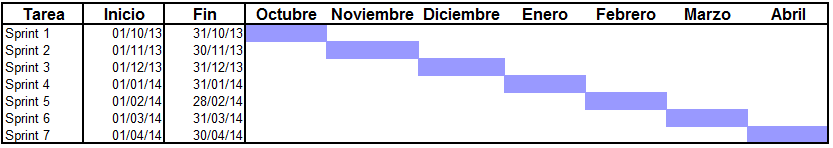
\includegraphics[width=0.9\linewidth]{./Figures/Gantt.PNG}
\caption[Diagrama de Gantt]{Diagrama de Gantt}
\label{fig:Gantt}
\end{figure}

\subsubsection{Sprint 1}
Inicio del proyecto, establecer prioridades, documentarse etc. Lo que compone este sprint es:

\begin{itemize}
    \item Crear y configurar el repositorio Git y los clientes en los dos ordenadores.
    \item Leer la documentaci\'{o}n existente y obtener el c\'{o}digo fuente original.
    \item Iniciar dise\~{n}os gr\'{a}ficos preliminares en papel para elegir las bibliotecas 
    necesarias.
    \item Buscar y documentarse sobre las bibliotecas que cumplan los requisitos del punto 
    anterior. 
\end{itemize} 

\subsubsection{Sprint 2}
Una vez configurados ordenadores y elegidas las bibliotecas necesarias:

\begin{itemize}
    \item Reunirse con el cliente para realizar una captura de requisitos.
    \item Dise\~{n}ar unos prototipos funcionales.
    \item Documentar lo que se hab\'{i}a realizado hasta el momento, es decir, el tipo de 
    planificaci\'{o}n que se hab\'{i}a elegido,
    tecnolog\'{i}as que se iban a usar etc.
\end{itemize}

\subsubsection{Sprint 3}
El siguiente paso consiste en poder cargar v\'{i}deos, tantos como se quieran, desde el sistema de archivos.

\begin{itemize}
    \item Crear el control de cargar v\'{i}deos (contenedor de v\'{i}deos). El contenedor debe 
    permitir:
    \begin{itemize}
        \item Cargar distintos v\'{i}deos desde el sistema de archivos.
        \item Cada v\'{i}deo debe disponer de sus controles individuales. Play, pausa, stop y 
        avanzar de tantos segundos en tantos 
        segundos, poder silenciarlo, y que sea configurable por el usuario, mediante un archivo 
        de configuraci\'{o}n.
        \item El contenedor de v\'{i}deos debe disponer de unos controles generales que ofrezcan 
        id\'enticas funcionalidades
        que el punto anterior.
        \item Debe permitir establecer para cada v\'{i}deo el momento de inicio del v\'{i}deo 
        manualmente para mantener la 
        sincronizaci\'{o}n.
    \end{itemize}
\end{itemize}

\subsubsection{Sprint 4}
Despu\'{e}s de terminar la visualizaci\'{o}n de v\'{i}deos, lo siguiente en la lista de tareas es 
crear un visualizador de datos.

\begin{itemize}
    \item Crear el contenedor que nos permita ver datos. El control debe permitir:
    \begin{itemize}
        \item Visualizar datos continuos y discretos.
        \item Seleccionar un rango en la gr\'{a}fica, estableciendo un inicio y un fin para las 
        propiedades.
        \item Que muestre el progreso, y que este sincronizado con el v\'{i}deo.
        \item Guardar el inicio y fin seleccionado.
    \end{itemize}
\end{itemize}

\subsubsection{Sprint 5}
Ya tenemos todo preparado para funcionar, ahora hay que poder guardar datos.

\begin{itemize}
    \item Elegir el m\'etodo de guardado de los datos.
    \item Configurar la base de datos (si aplica).
    \item Crear el diagrama Entidad-Relaci\'{o}n que representara el modo de guardado de datos 
    (si aplica).
    \item A\~{n}adir al c\'{o}digo existente las llamadas necesarias a la base de datos (si 
    aplica).
    \item Permitir cambiar la ubicaci\'{o}n de la base de datos mediante un archivo de 
    configuraci\'{o}n (Si aplica).
\end{itemize}

\subsubsection{Sprint 6}
En este momento se dispone de una aplicaci\'{o}n completamente funcional pero con datos de 
prueba. 
Hay que poder cargar datos desde un origen de datos.

\begin{itemize}
    \item Crear la clase para interactuar con el origen de datos.
    \item Hablar con el cliente para saber como est\'{a}n guardados los datos.
    \item Utilizando los datos de origen cargar la aplicaci\'{o}n con esos datos.
\end{itemize}

\subsubsection{Sprint 7}
Este \'ultimo sprint es sobre todo para hablar con el cliente para
ver si sus requisitos iniciales satisfacen sus necesidades actuales
y terminar la documentaci\'on as\'i como una revisi\'on general del c\'odigo
para posibles optimizaciones, refactorizado final, a\~nadir o quitar comentarios
en funci\'on de su necesidad.

Tambi\'en se finalizar\'a la documentaci\'on y memoria para dejarla para ser presentada.

Este sprint final es para dar por cerrado el proyecto.

\section{Herramientas}
El TFG al requerir de una cierta compatibilidad con el proyecto
existente, no se ha tenido libertad total en 
elecci\'on de herramientas. 

Las herramientas que se han utilizado para llevar a cabo este proyecto han sido:
\begin{itemize}
    \item 
    \textbf{Visual Studio}
    El \'unico software en el que no se ha tenido libertad de elecci\'on. Debido a que el 
    software en el que este TFG
    ser\'a integrado est\'a desarrollado usando Visual Studio, se ha utilizado por 
    compatibilidad. Adem\'as, se estaba
    valorando la posibilidad de portar el software original a WPF por lo que Visual Studio se 
    convert\'ia en una elecci\'on
    obvia ya es un software muy potente dise\~nado para trabajar e integrarse perfectamente con 
    esas tecnolog\'ias.

    La versi\'on utilizada ha sido Visual Studio 2013 Ultimate, proporcionado de manera gratuita 
    gracias al acuerdo que mantiene 
    la UPV/EHU con Microsoft.
    
    \item 
    \textbf{TeXstudio y \LaTeX}
    
    Dos herramientas gratuitas y de código abierto para generar documentos con el lenguaje de 
    programaci\'on \LaTeX.
    
    \item
    \textbf{Git y GitHub}
    
    Fundamental en los proyectos que se basen en metodologías ágiles. Git es un software de 
    gestión de control de versiones 
    distribuido, esto es, que cada desarrollador dispone de una copia completa del repositorio, 
    desarrollado por Linus Torvalds y 
    Junio Hamano en 2005 y similar a SVN.
    
    GitHub es un repositorio online, gratuito para proyectos Open Source desarrollado y mantenido 
    por GitHub Inc. Se ha elegido
    por ser la alternativa m\'as conocida as\'i como punto de referencia de los desarrolladores a 
    la hora de alojar proyectos.
    
\end{itemize}

\section{Gesti\'{o}n de riesgos}
Como en todo proyecto de software, existen una serie de riesgos que hay que tener en cuenta y en 
la medida de lo posible,
evitarlos. Es por ello que se necesita tener en cuenta las probabilidades de los sucesos que 
pueden ocurrir y que puedan retrasar el trabajo de forma notable. Una vez
listados, se puede proceder a crear un plan de prevención para evitarlos. Y en caso de que la 
prevenci\'on no
funcionase, un plan de contingencia que pueda amortiguar las consecuencias de ese riesgo. A 
continuación
se listan de forma detallada los riesgos que pueden aparecer durante el transcurso del proyecto.

\subsection{Planificaci\'{o}n}
En esta categor\'{i}a se engloban los riesgos que pueden causados por una mala planificaci\'{o}n 
temporal.
\subsubsection{Mala concepci\'{o}n del proyecto}
\begin{table}[H]
    \begin{center}
       \rowcolors{1}{lightgray}{} %\rowcolors{<starting row index>}{<odd row color>}{<even row color>}
       \begin{tabular}{l p{8cm}}
           Descripci\'{o}n                 & Por decisiones erróneas, como puede ser elegir 
           utilizar una
           base de datos, puede que el trabajo deba ser reconstruido desde el principio. \\
           Prevenci\'{o}n                  & Una buena planificación y conocimiento exacto de lo 
           que quiere y necesita el cliente. 
           									  \\ 
           Plan de contingencia            & Un programa flexible a cambios. \\
           Probabilidad                    & Improbable. \\
           Impacto                         & Muy alto. \\
        \end{tabular}
    \end{center}
    
\end{table}
\subsubsection{Error en la planificaci\'{o}n temporal}
\begin{table}[H]
    \begin{center}
        \rowcolors{1}{lightgray}{} %\rowcolors{<starting row index>}{<odd row color>}{<even row color>}
        \begin{tabular}{l p{8cm}}
            Descripci\'{o}n                 & Por una mala compresi\'on y falta de experiencia el 
            c\'alculo
            de tiempo estimado de una de las tareas es err\'oneo y hay que reajustar todo el 
            proyecto. \\
            Prevenci\'{o}n                  & Realizar la estimación lo mejor posible y tener una 
            buena
            								  comunicaci\'on con el cliente para no tener fallos 
            								  de comprensión. Utilizar de manera 
            								  correcta las metodolog\'ias \'agiles. \\ 
            Plan de contingencia            & Margen de error en los tiempos. \\
            Probabilidad                    & Muy probable. \\
            Impacto                         & Medio. \\
        \end{tabular}
    \end{center}
    
\end{table}
\subsection{Entorno de desarrollo}
\subsubsection{Incompatibilidad de versiones}
\begin{table}[H]
    \begin{center}
        \rowcolors{1}{lightgray}{} %\rowcolors{<starting row index>}{<odd row color>}{<even row color>}
        \begin{tabular}{l p{8cm}}
            Descripci\'{o}n                 & Al utilizar dos ordenadores, una workstation y un port\'{a}til puede que no 
            								  disponga de las mismas versiones del software o que no se satisfagan todas las 
            								  dependencias. \\
            Prevenci\'{o}n                  & Asegurarse de disponer el mismo software con las mismas versiones. \\ 
            Plan de contingencia            & Resolver manualmente las dependencias. \\
            Probabilidad                    & Probable \\
            Impacto                         & Bajo\\
        \end{tabular}
    \end{center}
    
\end{table}
\subsubsection{Problemas con GIT}
\begin{table}[H]
    \begin{center}
        \rowcolors{1}{lightgray}{} %\rowcolors{<starting row index>}{<odd row color>}{<even row color>}
        \begin{tabular}{l p{8cm}}
            Descripci\'{o}n                 & Al ser algo no ense\~{n}ado en profundidad en la universidad puede causar problemas al 
            								  usar las funciones avanzadas. \\
            Prevenci\'{o}n                  & Tener un buen manual y tener una copia local en otra carpeta para prevenir perdidas de 
            								  informaci\'{o}n. \\ 
            Plan de contingencia            & Desechar el software de control de versiones y buscar alternativas como Dropbox. \\
            Probabilidad                    & Poco probable \\
            Impacto                         & Bajo \\
        \end{tabular}
    \end{center}  
\end{table}
\subsubsection{Problemas con las librer\'{i}as}
\begin{table}[H]
    \begin{center}
        \rowcolors{1}{lightgray}{} %\rowcolors{<starting row index>}{<odd row color>}{<even row color>}
        \begin{tabular}{l p{8cm}}
            Descripci\'{o}n                 & Que las librer\'{i}as escogidas no cumplan los requisitos necesarios \\
            Prevenci\'{o}n                  & Mirar con anterioridad que s\'i los cumplan. \\ 
            Plan de contingencia            & Buscar una alternativa o intentar parchear la actual, ya que son de c\'{o}digo 
            								  abierto. \\
            Probabilidad                    & Muy probable \\
            Impacto                         & Alto \\
        \end{tabular}
    \end{center}
    
\end{table}
\subsection{Usuarios finales y clientes}
\subsubsection{No agrado del producto}
\begin{table}[H]
    \begin{center}
        \rowcolors{1}{lightgray}{} %\rowcolors{<starting row index>}{<odd row color>}{<even row color>}
        \begin{tabular}{l p{8cm}}
            Descripci\'{o}n                 & Despu\'{e}s de la entrega del proyecto puede suceder que el cliente no est\'{e} 
            								  satisfecho. \\
            Prevenci\'{o}n                  & Una buena comunicación con el cliente y reuniones progresivas para ir mostrando la 
            								  evolución del proyecto. \\ 
            Plan de contingencia            & Blindar las caracter\'{i}sticas, solo se realizaran las estipuladas durante el 
            							   	  proyecto. \\
            Probabilidad                    & Probable \\
            Impacto                         & Muy alto \\
        \end{tabular}
    \end{center}
    
\end{table}

\subsubsection{Manejo poco intuitivo}
\begin{table}[H]
    \begin{center}
        \rowcolors{1}{lightgray}{} %\rowcolors{<starting row index>}{<odd row color>}{<even row color>}
        \begin{tabular}{l p{8cm}}
            Descripci\'{o}n                 & Como  los  programadores  tienen  un  conocimiento
            inform\'{a}tico superior no tendr\'{a}n problemas con el uso, pero los usuarios si pueden tenerlos.\\
            Prevenci\'{o}n                  & Un diseño de interfaz sencillo y probar versiones con
            usuarios con conocimientos inform\'{a}ticos bajos. \\ 
            Plan de contingencia            & Adaptar la interfaz en el siguiente sprint. \\
            Probabilidad                    & Probable. \\
            Impacto                         & Alto \\
        \end{tabular}
    \end{center}
    
\end{table}

\subsection{Personas}
\subsubsection{Bajas por enfermedad}
\begin{table}[H]
    \begin{center}
        \rowcolors{1}{lightgray}{} %\rowcolors{<starting row index>}{<odd row color>}{<even row color>}
        \begin{tabular}{l p{8cm}}
            Descripci\'{o}n                 & El \'{u}nico componente del equipo cae enfermo y no puede trabajar. \\
            Prevenci\'{o}n                  & No existe prevenci\'{o}n. \\ 
            Plan de contingencia            & Recuperarse lo antes posible y manejar cierta holgura con las fechas.\\
            Probabilidad                    & Probable. \\
            Impacto                         & Muy alto \\
        \end{tabular}
    \end{center}
    
\end{table}

\subsection{Requisitos}
\subsubsection{Nuevos requisitos}
\begin{table}[H]
    \begin{center}
        \rowcolors{1}{lightgray}{} %\rowcolors{<starting row index>}{<odd row color>}{<even row color>}
        \begin{tabular}{l p{8cm}}
            Descripci\'{o}n                 & Debido a que el cliente tiene nuevas necesidades solicita la
            								  implementaci\'{o}n de funcionalidades extras o la desaparici\'{o}n de alguna que se 
            								  hayan podido volver innecesarias. \\
            Prevenci\'{o}n                  & Realizar un buen dise\~{n}o para que la posibilidad de añadir
            								  funcionalidades no suponga un coste muy elevado. \\ 
            Plan de contingencia            & Evaluar los nuevos requisitos para saber si se pueden
            								  abordar o no y si fuese que s\'i estudiar la situación y realizarlo. \\
            Probabilidad                    & Probable \\
            Impacto                         & Alto \\
        \end{tabular}
    \end{center}
    
\end{table}

\subsubsection{Requisitos no contemplados (ocultos)}
\begin{table}[H]
    \begin{center}
        \rowcolors{1}{lightgray}{} %\rowcolors{<starting row index>}{<odd row color>}{<even row color>}
        \begin{tabular}{l p{8cm}}
            Descripci\'{o}n                 & Requisitos explícitos desde el principio, pero que no fueron
            vistos en el primer an\'{a}lisis y al verlos en un futuro, provocan cambios en todos los niveles. \\
            Prevenci\'{o}n                  & Utilizar correctamente Scrum. \\ 
            Plan de contingencia            & A\~{n}adirlo como una tarea al siguiente sprint. \\
            Probabilidad                    & Muy probable. \\
            Impacto                         & Medio-Bajo. \\
        \end{tabular}
    \end{center}
    
\end{table}

\section{Planificaci\'{o}n econ\'{o}mica}
Debido a que el software creado va a ser donado a un grupo de investigaci\'on, todos los datos
utilizados en esta secci\'on de la planificaci\'on econ\'omica se han realizado suponiendo
que el proyecto se realiza al amparo del grupo de investigaci\'on como personal contratado y que se va a pedir
financiaci\'on al Gobierno Vasco.

Al realizar esta suposici\'on, es necesario crear una estimaci\'on de los costes para poder
pedir la ayuda al gobierno y de esta forma llevar a cabo el proyecto.

\subsection{Ingresos}
No se obtendr\'{a} beneficio econ\'{o}mico del proyecto ya que se realiza con car\'acter comunitario y con la intenci\'on
de ayudar a un grupo de investigaci\'on. El c\'odigo est\'a disponible y ser\'a liberado bajo licencia GPLv3.

Por lo tanto el coste de venta de nuestro coste sera 0€ as\'i como los ingresos directos obtenidos por el software.

\subsection{Salario del investigador responsable}
Teniendo en cuenta la complejidad, y el tiempo disponible para realizar el software, se ha
decidido dar un salario compensatorio de 30 € / hora al responsable desarrollador del proyecto.

Para calcular el salario total a percibir, se ha utilizado la cantidad estimada media de horas
que se le dedicar\'a al proyecto, que son 60 horas / mes.
Por tanto:

\begin{center}
	$ Total \ horas = 60 horas / mes * 7 meses = 420 horas $
	
	$ Total \ a \ percibir (€) = 420 horas * 30 € / hora = 12600 € $
\end{center}

\subsubsection{Lugar de trabajo}
El lugar de trabajo es el domicilio familiar y no hay que pagar alquiler ya que est\'a en
propiedad. Por lo que el gasto de alquiler/hipoteca es 0€.

\subsection{Amortizaci\'on material inform\'atico}
Con la amortizaci\'on cargamos al cliente con el desgaste que supone utilizar esos
dispositivos para esa tarea. Como el proyecto ha durado siete meses, la amortizaci\'on
correspondiente a este a\~no deber\'a ser multiplicada por $ \frac{7 meses}{12 meses} = 0.582 $ 
para cobrar de manera correcta por ese desgaste. Este factor se le aplicar\'a tanto al Software de pago como
a los dispositivos inform\'aticos utilizados.

\subsubsection{Material inform\'{a}tico}
El material informático que se va a usar es un portátil Acer TravelMate 5742G comprado en 
Diciembre de 2010 y usado intensivamente durante estos 4 años. 
El portátil estaba pensado para ser amortizado en 8 años.

Por lo tanto:

El coste del port\'atil fue de 549€ IVA incluido.
\begin{center}
\begin{equation}
Amortizacion \ anual (\%) = \frac{100}{8} = 12.5 \%
\end{equation}

\begin{equation}
Amortizacion \ anual (€) = \frac{Amortizacion \ anual(\%) * Precio \ dispositivo}{100}
\end{equation}

\begin{equation}
Amortizacion \ anual (€) = \frac{12.5 * 549}{100} = 68.625 €
\end{equation}

\begin{equation}
Amortizacion \ a \ cargar (€) = 68.625 * 0,583 = 39.79 €
\end{equation}


\begin{equation}
Amortizacion \ acumulada (€) = 68.625 * 4 = 274.5 €
\end{equation}

\begin{equation}
Amortizacion \ acumulada (2014) = 274.5 + 68.625 = 343.125 €
\end{equation}

\end{center}

Tambi\'{e}n se va a usar un PC gen\'{e}rico comprado a piezas en 2012, y pensado para
ser amortizado en 10 a\~nos. El precio fue 277.65 € IVA incluido.
Por lo que su amortizaci\'on hasta el d\'ia de hoy ha sido:

\begin{center}
\begin{equation}
Amortizacion \ anual (\%) = \frac{100}{10} = 10.0 \%
\end{equation}

\begin{equation}
Amortizacion \ anual (€) = \frac{Amortizacion \ anual(\%) * Precio \ dispositivo}{100}
\end{equation}

\begin{equation}
Amortizacion \ anual (€) = \frac{10.0 * 277.65}{100} = 27.765 €
\end{equation}

\begin{equation}
Amortizacion \ a \ cargar (€) = 27.765 * 0.583 = 16.187 €
\end{equation}

\begin{equation}
Amortizacion \ acumulada (€) = 27.765 * 2 = 55.53 €
\end{equation}

\begin{equation}
Amortizacion \ acumulada (2014) = 55.53 + 27.765 = 83.295 €
\end{equation}

\end{center}

\subsection{Software}
Debido a la previa suposici\'on de que se est\'a trabajando de manera conjunta con la 
universidad como personal contratado, se hace necesario contabilizar como gasto las licencias de software.

\subsubsection{Visual Studio}
La versi\'on de Visual Studio utilizada es la 2013 Ultimate, la m\'as completa y a la vez m\'as
cara, y que su Precio de Venta al P\'ublico, es de 14.237,91€ \footnote{\url{http://www.visualstudio.com/en-us/products/visual-studio-ultimate-with-msdn-vs\#Fragment_PricingHeader}}.

Como es un software muy caro, se le va a aplicar una amortizaci\'on de 4 a\~nos.
Parece poco tiempo, pero en t\'erminos de desarrollo es un periodo bastante largo, y adem\'as
Microsoft ofrece unos precios razonables de actualizaci\'on.

\begin{center}
\begin{equation}
Amortizacion \ anual (\%) = \frac{100}{4} = 25.0 \%
\end{equation}

\begin{equation}
Amortizacion \ anual (€) = \frac{Amortizacion \ anual(\%) * Precio \ software}{100}
\end{equation}

\begin{equation}
Amortizacion \ anual (€) = \frac{25.0 * 14237.91 €}{100} = 3559.4775 €
\end{equation}

\begin{equation}
Amortizacion \ a \ cargar (€) = 3559.4775 * 0.583 = 2075.17 €
\end{equation}

\begin{equation}
Amortizacion \ acumulada (€) = 3559.4775 * 0 = 0 €
\end{equation}

\begin{equation}
Amortizacion \ acumulada (2014) = 0 + 3559.4775 = 3559.4775 €
\end{equation} 
\end{center} 

\subsubsection{Resto del software}
El resto del software utilizado es gratuito y de c\'odigo abierto, por lo que no contiene
ning\'un tipo de gasto.

\subsection{Otros gastos}
Los gastos comunes del proyecto (Agua, Internet, Luz, Gas) supondr\'an un 5\% del coste
total del proyecto.

\subsection{Gastos totales}
La tabla \ref{GastosTotales} resume los gastos estimados del proyecto,
aquellos gastos que son 0€ no se a\~naden a la tabla.
\begin{table}[H]
	\begin{center}
		\begin{tabular}{l*{1}{r}r}
		    Concepto                   & Gastos en € & \\
		    \hline
		    Amortizaci\'on material    & 55,977  & \\
		    Gastos personal (salario)  & 12.600,000 & \\
		    Software                   & 2.075.170 & \\
		    \hline
		    Sub total				   & 14.062,290 & \\
		    \hline
		    Gastos comunes			   & 1.203,115 & \\
		    \hline
		    Total		               & 25.265,410 &\\
		\end{tabular}
	\caption[Gastos totales]{Gastos totales}
	\label{GastosTotales}
	\end{center}
\end{table}

